\documentclass [12pt, a4paper] {article}

%Babel tekee kuulemma jotain typer��, joten seuraava on v�ltt�m�t�nt�.
\usepackage[all, knot] {xy}
\let\oldxy\xy\def\xy{\begingroup\catcode`\"12\oldxy}
\let\oldendxy\endxy\def\endxy{\oldendxy\endgroup} 
\xyoption {arc}
\usepackage [latin1] {inputenc}
\usepackage [T1] {fontenc}
\usepackage [english] {babel}
\usepackage [dvips] {graphicx}
\usepackage {amsfonts}
\usepackage {amssymb}
\usepackage {amsmath}
\usepackage {verbatim}
\usepackage {fancyhdr}
\usepackage {psfrag}
\usepackage {listings}
\usepackage {eso-pic}
\usepackage {siunitx}
\usepackage {wasysym}
\usepackage {marvosym}
%\usepackage {mathabx}
%\usepackage[urw-garamond]{mathdesign}
\usepackage[small,bf]{caption}
\usepackage{enumitem}
\usepackage{stix}
\usepackage{lipsum}
\usepackage{tikz}
\usetikzlibrary{arrows.meta}
\usepackage{hyperref}
\usepackage[dvipsnames]{xcolor}

\newcommand{\BackgroundPic}{
%  \put(0,0){
%    \parbox[b][\paperheight]{\paperwidth}{
%      \vfill
%      \centering
%      \includegraphics[width=\paperwidth, height=\paperheight, keepaspectratio%]{
%kansilehti.ps}
%    }
%  }
%  \textbf{SMG-5156 - Electromagnetic Modelling I}\\
%  \textbf{Exercise 1 - Problem 4}\\
%  \textbf{Ville R�is�nen}
%\end {flushleft}

%  \put(42, 810){\textbf{SMG-5156 - Electromagnetic Modelling I}}
%  \put(42, 797){\textbf{Exercise 1 - Problem 1}}
%  \put(42, 784){\textbf{Ville R�is�nen}}
%  \put(445, 810){\textbf{Please, do not distribute!}}
}

\addtolength{\evensidemargin}{-1cm}
\addtolength{\oddsidemargin}{-1cm}
\addtolength{\marginparwidth}{-2.0cm}
\addtolength{\topmargin}{-2cm}
\addtolength{\textwidth}{3cm}
\addtolength{\textheight}{2cm}
\addtolength{\columnsep}{0.5cm}

 
\lhead {Optical Effects from Observer Motion\\Ville R{\"a}is{\"a}nen (\url{https://www.github.com/vsr83})}
\rhead {\today}
\thispagestyle{fancy}

\newtheorem {problem} {Problem}
\newtheorem {example} {Example}
\newtheorem {theorem} {Theorem}
\newtheorem {definition} {Definition}
\newtheorem {postulate} {Postulate}

\newcommand{\vu}[1]
{
	\mathbf{\hat #1}
}
\newcommand{\vf}[1]
{
	\mathbf{\vec #1}
}
\newcommand{\mc}[1]
{
	\mathcal{#1}
}
\newcommand{\vc}[1]
{
	\boldsymbol{#1}
}
\newcommand{\vcc}[1]
{
	\widetilde{\boldsymbol{#1}}
}
\newcommand{\cc}[1]
{
	\widetilde{#1}
}
\newcommand{\sgn}
{
  \textrm{sgn}\:
}
\newcommand{\pdiff}[2]
{
	\dfrac{\partial #1}{\partial #2}
}
\newcommand{\diff}[2]
{
	\dfrac{d #1}{d #2}
}
\newcommand{\vali}
{
  \begin {displaymath}\:\end{displaymath}
}
\newcommand{\norm}[2]
{
  ||#1||_{#2}
}

\newcommand{\solution}
{
   {\textbf{\textrm{Solution:}}}
}
\newcommand{\motivation}
{
  {\textbf{\textrm{Motivation:}}}
}

\begin {document}

\tableofcontents

\newpage

\section{Aberration Formulas}
\subsection {Classical and Relativistic Aberration}
\begin {figure}[t]
  \begin {center}
    \begin{tikzpicture}
        \draw[thick, color=gray!50] (3.5, 0) -- (4, 0.5);
        \draw[thick, color=gray!50] (3, 0) -- (4, 1);
        \draw[thick, color=gray!50] (3, 0.5) -- (4, 1.5);
        \draw[thick, color=gray!50] (3, 1) -- (4, 2);
        \draw[thick, color=gray!50] (2, 0.5) -- (3.5, 2);
        \draw[thick, color=gray!50] (2.0, 1) -- (3.0, 2);
        \draw[thick, color=gray!50] (1.5, 1) -- (2.5, 2);
        \draw[thick, color=gray!50] (0.0, 0) -- (2.0, 2);
        \draw[thick, color=gray!50] (0.0, 0.5) -- (1.5, 2);
        \draw[thick, color=gray!50] (0.0, 1.0) -- (1.0, 2);
        \draw[thick, color=gray!50] (0.0, 1.5) -- (0.5, 2);

        \draw[thick, color=gray!50] (9.0, 0) -- (10, 0.5);
        \draw[thick, color=gray!50] (8.0, 0) -- (10, 1.0);
        \draw[thick, color=gray!50] (7.0, 0) -- (10, 1.5);
        \draw[thick, color=gray!50] (7.0, 0.5) -- (10, 2);
        \draw[thick, color=gray!50] (6.0, 0.5) -- (9, 2);
        \draw[thick, color=gray!50] (6.0, 1) -- (8, 2);
        \draw[thick, color=gray!50] (6.0, 1.5) -- (7, 2);


        \draw[fill=gray!10] (1,0) rectangle (3,1);
        \draw[thick] (0, 0) -- (4, 0);
        \draw[fill=gray!10] (7,0) rectangle (9,1);
        \draw[thick] (6, 0) -- (10, 0);
        \draw[thick] (8, 0) -- (10, 1);

        \draw[thick, ->] (2, 0) -- (2, 1.5);
        \draw[thick, ->] (2, 0) -- (3.5, 0);
        \draw[thick, ->] (8, 0) -- (8, 1.5);
        \draw[thick, ->] (8, 0) -- (9.5, 0);
        \draw[thick] (2, 0) -- (4, 2);
        \draw[thick] (2.4,0) arc (0:45:0.4);
        \draw[thick] (8.5,0) arc (0:25:0.5);
        \draw (2.6,0.25) node{$\theta$};
        \draw (8.9,0.25) node{$\theta'$};
        \draw[thick, ->] (3, 0.5) -- (4, 0.5);
        \draw (3.5,0.75) node{$v$};

        \draw (1.65,1.25) node{$y$};
        \draw (3.35,-0.35) node{$x$};
        \draw (7.65,1.25) node{$y'$};
        \draw (9.35,-0.305) node{$x'$};


        \draw (0,0.5) node{$S$};
        \draw (6,0.5) node{$S'$};
    \end {tikzpicture}
    \caption{\label{fig:train}Path of the rain drops in a frame fixed to the ground and 
    the train.}
  \end {center}
\end {figure}
Consider a train cart fixed to the frame $S'$ moving in $+x$-direction with velocity 
$v$ w.r.t. frame $S$ fixed to the ground. Passenger on the train observes the direction 
of rain drops from the window. Suppose in $S$ it is raining from direction 
$\theta$ w.r.t. the positive x axis. Then, the path of rain drop falling through $x=y=0$ 
can be written
\begin {eqnarray}
    x(t) &=& -u\cos\theta\:t,\\
    y(t) &=& -u\sin\theta\:t,
\end {eqnarray}
where $u$ is the velocity of the rain drop in $S$. In $S'$, we can express
\begin {eqnarray}
    x'(t) &=& -(u\cos\theta + v)t,\\
    y'(t) &=& -u(\sin\theta)t.
\end {eqnarray}
In $S'$, the angle $\theta'$ made by the rain drops w.r.t. positive x axis can be 
expressed 
\begin {eqnarray}
    \tan\theta' 
    = 
    \frac{y'}{x'} 
    =
    \frac{u\sin\theta}{u\cos\theta + v} 
    =
    \frac{\tan\theta}{1 + \beta\sec\theta},
\end {eqnarray}
where $\beta = v/u$ and $\sec\theta = 1/\cos\theta$. This classical formula is 
limited angles in $+x$ direction. More generally,
\begin {eqnarray}
    \theta' 
    =
    \textrm{atan2}(\sin\theta, \cos\theta + \beta) 
\end {eqnarray}

\begin {figure}
  \begin {center}
     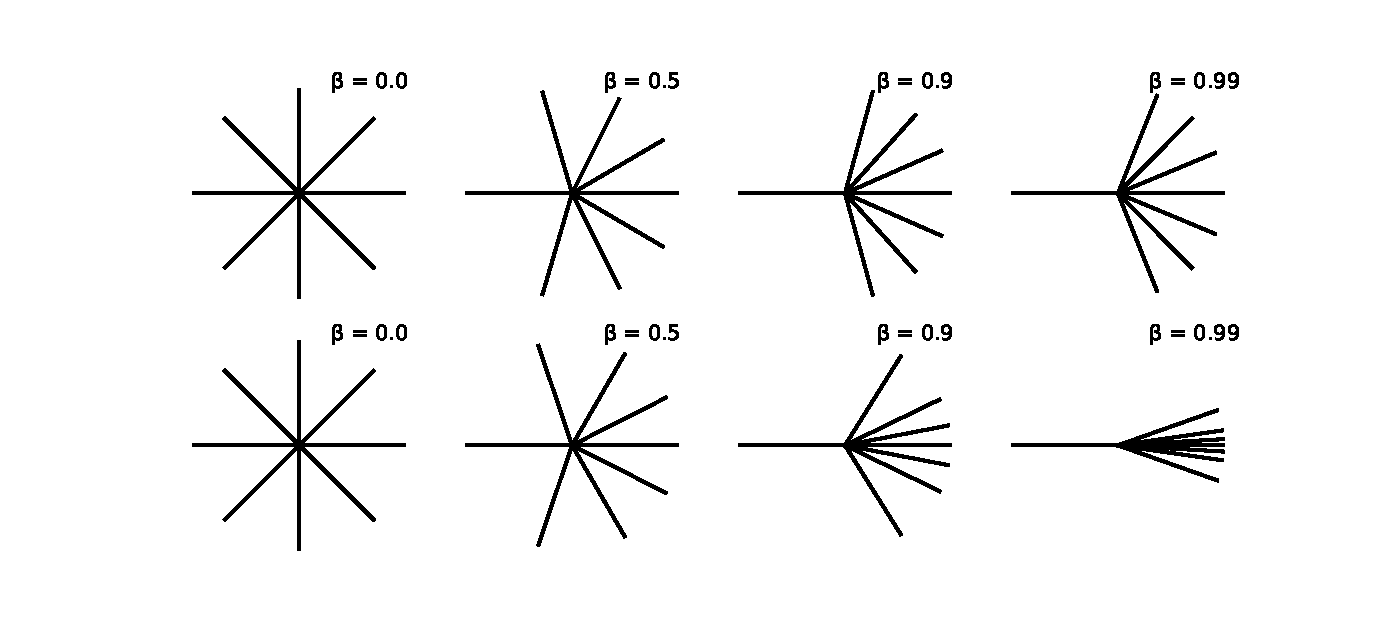
\includegraphics [angle=0, width=0.9\columnwidth] {fig/aberration.eps}
     \caption{\label{fig:classicrel}Difference between classical (top) and relativistic 
     (bottom) aberration.}
  \end {center}
\end {figure} 
Consider now light in the context of Special Relativity with velocity vector 
$\vc c = (-c\cos\theta, -c\sin\theta, 0)$. Then, simple application of Lorentz 
transformation, yields 
\begin {eqnarray}
    x' &=& \gamma(x - vt) 
    = -\gamma(c\cos\theta + v) t,
    \\
    y' &=& y = -(c\sin\theta)t,
\end {eqnarray}
where the \textbf{Lorentz factor} is defined
\begin {eqnarray}
    \gamma:
    = 
    \frac{1}{\sqrt{1 - v^2/c^2}}
    =
    \frac{1}{\sqrt{1 - \beta^2}}.
\end {eqnarray}
Thus, we obtain the well-known formula for relativistic aberration
\begin {eqnarray}
    \tan\theta' = \frac{y'}{x'} = \frac{\tan\theta}{\gamma(1 + \beta\sec\theta)}
\end {eqnarray}
and the more general expression
\begin {eqnarray}
    \theta' 
    =
    \textrm{atan2}\left[\sin\theta, \gamma(\cos\theta + \beta)\right]
\end {eqnarray}
The only difference between classical and relativistic aberration is the Lorentz 
factor. When $\beta$ is small, the difference between relativistic and classical 
results can be usually ignored. At velocities close to the speed of light, the 
Lorentz factor leads to light sources accumulating around direction of motion 
(see Figure \ref{fig:classicrel}).

\begin {figure}
  \begin {center}
     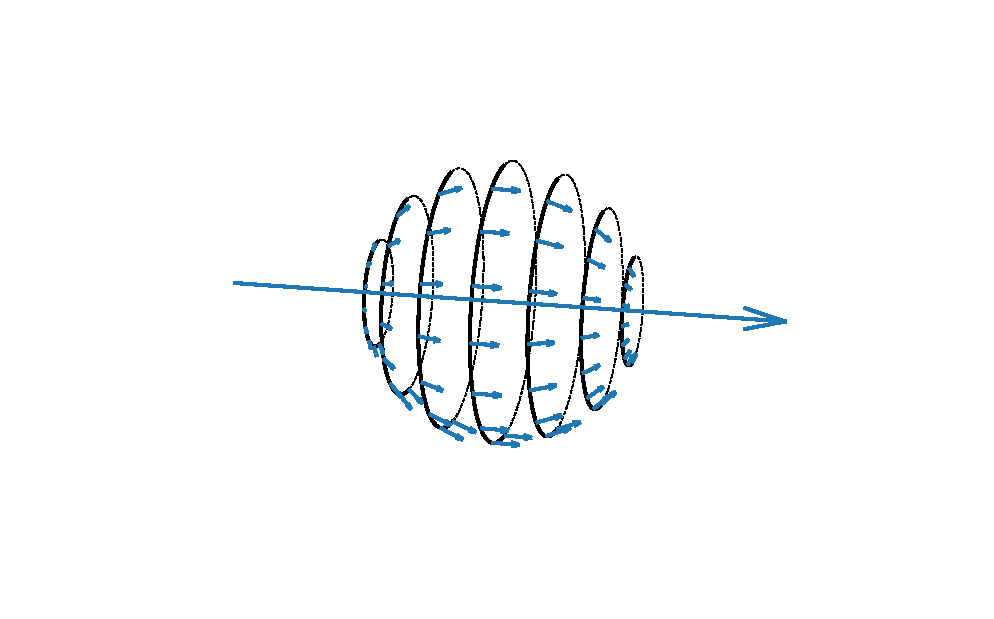
\includegraphics [angle=0, width=0.6\columnwidth, viewport=100 70 370 220, clip=true] {fig/aberration3d.eps}
     \caption{\label{fig:3d} Three-dimensional depiction of the aberration 
     correction for a velocity vector and the associated rotational symmetry.}
  \end {center}
\end {figure} 



\subsection{General Vector Expression for Aberration}
For practical computations, it is often more convenient to use vectors. Any 
vector expression for aberration will involve addition of velocity vectors,
which is non-trivial in relativistic case.
\subsubsection{Classical Aberration}
In the classical case, the transformation of velocities is simply 
\begin {eqnarray}
    \label{eq:classicaladd}
    \vc u' = \vc u - \vc v.
\end {eqnarray}
The direction to target $\vu s = -\vc u'/|\vu u'|$ corrected for aberration is 
called the \textbf{proper direction}. Unlike the relativistic expression
$\vu s = -\vc u'/c$ , the 
classical expression for the proper direction needs to take into account that 
classical addition of velocities can lead to velocity of light greater than 
$c$. The \textbf{uncorrected direction} in both cases can be written 
$\vu p = -\vu u/c$. 

Direct substitution to $(\ref{eq:classicaladd})$, yields
\begin {eqnarray}
    -\vu s|c\vu p + \vc v|
    =
    -c\vu p - \vc v
\end {eqnarray}
and denoting $\vc\beta = \vc v/c$, we obtain the classical vector expression 
for proper direction
\begin {eqnarray}
    \label{eq:classical_properdir}
    \boxed{
        \quad
        \vu s
        =
        \frac{\vu p + \vc v/c}{|\vu p + \vc v/c|}
        =
        \frac{\vu p + \vc\beta}{|\vu p + \vc\beta|}
        \quad
    }.
\end {eqnarray}

\subsubsection{General Lorentz Transformation of Velocities}
Let $S'$ move w.r.t. $S$ with velocity $\vc v$ and denote 
\begin {eqnarray}
    \vc u := \diff{\vc r}{t}, 
    \quad
    \vc u' := \diff{\vc r'}{t'},.
\end {eqnarray}
Then, the Lorentz transformation will only affect coordinates along the direction 
of the velocity. That is, parallel and perpendicular components of $d\vc r$ 
transform as
\begin {eqnarray}
    d\vc r_{||}' &=& \gamma\left(d\vc r_{||} - \vc v\:dt\right)
    \\
    d\vc r_{\perp}' &=& d\vc r_\perp.
\end {eqnarray}
The time transforms as 
\begin {eqnarray}
    dt' &=&
    \gamma\left(
        dt - \frac{\vc v\cdot d\vc r}{c^2}
    \right)
    =
    \gamma\left(
        1 - \frac{\vc v\cdot \vc u}{c^2}
    \right)dt.
\end {eqnarray}
Now we can expand the components of velocity in $S'$
\begin {eqnarray}
    \vc u_{||}'
    &=&
    \diff{\vc r_{||}'}{t'}
    = \frac{\gamma(\vc r_{||} - \vc v\:dt)}{\gamma(1 - \vc v\cdot\vc u/c^2)dt}
    = \frac{\vc u_{||} - \vc v}{1 - \vc v\cdot\vc u/c^2}
    \\
    \vc u_{\perp}'
    &=&
    \diff{\vc r_{\perp}'}{t'}
    =
    \frac{d\vc r_\perp}{\gamma(1 - \vc v\cdot\vc u/c^2)dt}
    =
    \frac{\vc u_\perp}{\gamma(1 - \vc v\cdot\vc u/c^2)}
\end {eqnarray}
The velocity in $S'$ can be expanded using 
\begin {eqnarray}
    \vc u_{||}=\frac{\vc u\cdot\vc v}{v^2}\vc v,
    \quad 
    \vc u_\perp = \vc u - \vc u_{||} = \vc u - \frac{\vc u\cdot\vc v}{v^2}\vc v
\end {eqnarray}
leading to 
\begin {eqnarray}
    \vc u' &=& \vc u_{||}' + \vc u_\perp'
    \\
    &=& 
    \frac{\vc u_{||} - \vc v + \vc u_\perp/\gamma}{1 - \vc v\cdot\vc u/c^2}
    \\
    &=& 
    \frac{1}{1 - \vc v\cdot\vc u/c^2}
    \left[
        \frac{\vc u\cdot\vc v}{v^2}\vc v 
        - \vc v
        + \frac{1}{\gamma}\left(
            \vc u - \frac{\vc u\cdot\vc v}{v^2}\vc v
        \right)
    \right]
    \\
    &=& 
    \frac{1}{1 - \vc v\cdot\vc u/c^2}
    \left\{
        \frac{1}{\gamma}\vc u
        +
        \vc v 
        \left[
             \frac{\vc u\cdot\vc v}{v^2}\left(1 - \frac{1}{\gamma}\right) - 1
        \right]
    \right\}
    \\
    \label{eq:vector_lorentz_vel}
    &=& 
    \frac{1}{\gamma(1 - \vc v\cdot\vc u/c^2)}
    \left[
        \vc u
        +
        \vc v 
        \left(
             \frac{\vc u\cdot\vc v}{v^2}\left(\gamma - 1\right) - \gamma
        \right)
    \right].
\end {eqnarray}


\subsubsection{Relativistic Aberration}
Let $\vu n= \vc u/c$ be the direction of light propagation and 
$\vu s = -\vc u'/c$ be the (relativistic) proper direction. Substitution to the
General Lorentz Transformation for velocities $(\ref{eq:vector_lorentz_vel})$ then 
yields 
\begin {eqnarray}
    -c\vu s 
    &=&
    \frac{1}{\gamma(1 - \vu n\cdot\vc v/c)}
    \left\{
        c\vu n
        +
        \vc v 
        \left[
             \frac{c}{v^2}(\vu n\cdot\vc v)\left(\gamma - 1\right) - \gamma
        \right]
    \right\}
\end {eqnarray}
or
\begin {eqnarray}
    \vu s 
    &=&
    \frac{1}{\gamma(1 - \vu n\cdot\vc v/c)}
    \left\{
        -\vu n
        +
        \vc v 
        \left[
             \frac{\gamma}{c} - \frac{1}{v^2}(\vu n\cdot\vc v)\left(\gamma - 1\right)
        \right]
    \right\}
    \\
    &=&
    \frac{1}{\gamma(1 - \vu n\cdot\vc v/c)}
    \left\{
        -\vu n
        +
        \vc v 
        \frac{\gamma}{c}
        \left[
             1 - \frac{c}{v^2}(\vu n\cdot\vc v)\frac{\gamma - 1}{\gamma}
        \right]
    \right\}
    \\
    &=&
    \frac{1}{\gamma(1 - \vu n\cdot\vc v/c)}
    \left[
        -\vu n
        +
        \vc v 
        \frac{\gamma}{c}
        \left(
             1 - \frac{\gamma}{\gamma + 1}\frac{\vc v\cdot\vu n}{c}
        \right)
    \right], 
\end {eqnarray}
where in the last step we have used 
\begin{eqnarray}
    \frac{\gamma - 1}{\gamma\beta^2} 
    &=&
    \frac{\gamma - 1}{\gamma(1 - \gamma^{-2})}
    =
    \frac{\gamma^2 - \gamma}{\gamma^2 - 1}
    =
    \gamma\frac{\gamma - 1}{(\gamma - 1)(\gamma + 1)}
    = \frac{\gamma}{\gamma + 1}
    \\
    \Rightarrow
    \frac{c}{v^2}\frac{\gamma - 1}{\gamma}(\vc v\cdot\vu n)
    &=& \frac{1}{c}\frac{\gamma - 1}{\gamma\beta^2}(\vc v\cdot\vu n)
\end {eqnarray}
Denoting $\vc\beta=\vc v/c$, we obtain expression for the proper direction
\begin {eqnarray}
    \label{eq:properdir1}
    \vu s 
    =
    \frac{1}{\gamma(1 - \vu n\cdot\vc\beta)}
    \left[
        -\vu n 
        + 
        \gamma\vc\beta 
        \left(
            1 - \frac{\gamma}{\gamma + 1}\vc\beta\cdot\vu n
        \right)
    \right]
\end {eqnarray}
Let $\vc p = -\vu n$ be the uncorrected direction. Then $(\ref{eq:properdir1})$ can 
be expressed 
\begin {eqnarray}
    \boxed{
        \quad
        \label{eq:properdir2}
        \vu s 
        =
        \frac{1}{\gamma(1 + \vu p\cdot\vc\beta)}
        \left[
            \vu p 
            + 
            \gamma\vc\beta 
            \left(
                1 + \frac{\gamma}{\gamma + 1}\vc\beta\cdot\vu p
            \right)
        \right].    
        \quad
    }
\end {eqnarray}

\subsection{Series Expansion of Aberration Correction}
\subsubsection{Classical Aberration}
Cross product of $(\ref{eq:classical_properdir})$ with uncorrected 
direction $\vc p$, yields
\begin {eqnarray}
    \sin\Delta\theta\:\vu n
    =
    \vu p\times\vu s 
    = 
    \frac{\vu p\times\vu p + \vu p\times\vc\beta}{|\vu p + \vc\beta|}
    = 
    \frac{\vu p\times\vc\beta}{|\vu p + \vc\beta|}
    = 
    \frac{||\vu p||\:||\vc\beta||\sin\theta\:\vu n}{|\vu p + \vc\beta|}
    = 
    \frac{\beta\sin\theta\:\vu n}{\sqrt{1 + 2\beta\cos\theta + \beta^2}},
\end {eqnarray}
where we have used 
\begin {eqnarray}
    ||\vu p + \vc\beta||^2
    &=&
    (||\vu p|| + ||\vc\beta||\cos\theta)^2 + \beta^2\sin^2\theta
    \\
    &=&
    1 + 2\beta\cos\theta + \beta^2\cos^2\theta + \beta^2\sin^2\theta 
    \\
    &=&
    1 + 2\beta\cos\theta + \beta^2.
\end {eqnarray}
According to generalized binomial theorem
\begin {eqnarray}
    \frac{1}{\sqrt{1 + x}} 
    = 
    \sum_{k=0}^\infty
    \binom{-1/2}{k}x^n 
    \approx 
    1 - \frac{1}{2}x + \frac{3}{8}x^2 - \frac{5}{16}x^3 + ...
\end {eqnarray}
Substitution of $x=2\beta\cos\theta + \beta^2$, yields
\begin {eqnarray}
    \frac{1}{\sqrt{1 + 2\beta\cos\theta + \beta^2}}
    &\approx&
    1 
    -
    \frac{1}{2}(2\beta\cos\theta + \beta^2)
    +
    \frac{3}{8}(2\beta\cos\theta + \beta^2)^2
    \\
    &=&
    1 - \cos\theta\beta 
    + 
    \left(\frac{3}{2}\cos^2\theta - \frac{1}{2}\right)\beta^2
    +
    \frac{3}{2}\cos\theta\beta^3 
    +
    \frac{3}{8}\beta^4
\end {eqnarray}
and if we ignore everything above fourth power of $\beta$, we can expand 
\begin {eqnarray}
    \sin\Delta\theta 
    \approx
    \beta\sin\theta 
    -
    \frac{1}{2}\beta^2\sin 2\theta
    +
    \frac{1}{8}\beta^3(3\sin 3\theta - \sin\theta)
    + 
    \frac{3}{4}\beta^4\sin 2\theta
\end {eqnarray}
Note that when such a series is expressed as a linear combination 
of sinusoidal terms, it is obvious that $\Delta\theta$ antisymmetric w.r.t. 
$\theta$ and zero at $\theta=0$. The above formula also produces a positive
$\Delta\theta$ with positive $\theta$, which is incorrect.
In most applications, where $\beta$ is small, we can approximate 
\begin {eqnarray}
    \label{eq:classical_series}
    \boxed{
        \quad
        \Delta\theta \approx\sin\Delta\theta \approx 
        -\beta\sin\theta + \frac{1}{2}\beta^2\sin 2\theta.
        \quad
    }
\end {eqnarray}

\subsubsection{Relativistic Aberration}
Cross product of $(\ref{eq:properdir2})$ with uncorrected direction $\vu p$, 
yields
\begin {eqnarray}
    ||\vu s||\:||\vu p||\sin\Delta\theta \vu n
    &=&
    \vu s\times\vu p 
    \\
    &=&
    \frac{\vc \beta\times\vu p}{1 + \vu p\cdot\vc\beta}
    \left(
        1 + \frac{\gamma}{\gamma + 1} \vc\beta\cdot\vu p
    \right)
    \\
    &=&
    \frac{\beta\sin\theta}{1 + \beta\cos\theta}
    \left(
        1 + \frac{\gamma}{\gamma + 1}\beta\cos\theta
    \right)
    \vu n.
\end {eqnarray}
To obtain a series expansion for $\sin\Delta\theta$, note that:
\begin {eqnarray}
    \frac{1}{1 + \beta\cos\theta}
    &=& 
    \sum_{k=0}^\infty(-1)^k \beta^k \cos^k\theta
    \approx 
    1 - \beta\cos\theta + \beta^2\cos^2\theta,
    \\
    \frac{\gamma}{\gamma + 1}
    &=&
    \frac{1}{1 + \sqrt{1 - \beta^2}}
    =
    \frac{1}{1 + \sqrt{1 - \beta^2}}
    \frac{1 - \sqrt{1 - \beta^2}}{1 - \sqrt{1 - \beta^2}}
    =
    \frac{1 - \sqrt{1 - \beta^2}}{\beta^2},
    \\
    \sqrt{1 - \beta^2} 
    &=&
    \sum_{k=0}^{\infty}
    \binom{1/2}{k}(-1)^k \beta^{2k}
    \approx 
    1 - \frac{1}{2}\beta^2 + \frac{1}{8}\beta^4.
\end {eqnarray}
Thus, we can also expand 
\begin {eqnarray}
  \frac{1 - \sqrt{1 - \beta^2}}{\beta^2}
    &\approx&
    \frac{1}{\beta^2}
    \left[
        1 - \left(1 - \frac{1}{2}\beta^2 + \frac{1}{8}\beta^4\right)
    \right]
    =
    \frac{1}{2} - \frac{1}{8}\beta^2,
    \\
    \beta\sin\theta\left(
        1 + \frac{\gamma}{\gamma + 1}\beta\cos\theta
    \right)
    &\approx&
    \beta\sin\theta + \beta^2\sin\theta\cos\theta 
    \left(
         \frac{1}{2} - \frac{1}{8}\beta^2
    \right)
    \approx
    \beta\sin\theta + \frac{1}{4}\beta^2\sin 2\theta\quad
\end {eqnarray}
and finally 
\begin {eqnarray}
    \sin\Delta\theta 
    &\approx&
    \left(1 - \beta\cos\theta\right)
    \left(\beta\sin\theta + \frac{1}{4}\beta^2\sin 2\theta\right)    
    \\
    &\approx&
    \beta\sin\theta - \beta^2\sin\theta\cos\theta + \frac{1}{4}\beta^2\sin 2\theta
\end {eqnarray}
Thus, again noting the sign, we obtain the approximation
\begin{eqnarray}
    \label{eq:relativistic_series}
    \boxed{
        \quad
        \Delta\theta
        \approx
        \sin\Delta\theta
        \approx
        -\beta\sin\theta + \frac{1}{4}\beta^2\sin 2\theta.
        \quad        
    }
\end {eqnarray}
\subsubsection{Accuracy}
The difference in the quadratic term between $(\ref{eq:relativistic_series})$ 
and $(\ref{eq:classical_series})$ suggests that the linear approximation can be
more preferrable than the quadratic classical approximation. 
Comparison with two values of $\theta$ is shown in Figure \ref{fig:series}.
Worst case (w.r.t. $\theta$) relative errors are shown in Figure \ref{fig:error}.

The linear approximation is usually sufficient for most purposes in astrometry:
For example, if Earth's speed along it's orbit is about $30$ km/s or 
$\beta\approx 10^{-4}$, the maximum relative error from linear and quadratic 
approximations are on the scale of $10^{-4}$ and $10^{-8}$, respectively. If the 
maximum aberration is around $20$", this corresponds to absolute errors 
around $2$ mas and $0.2$ $\mu$as, respectively.

\begin {figure}
  \begin {center}
     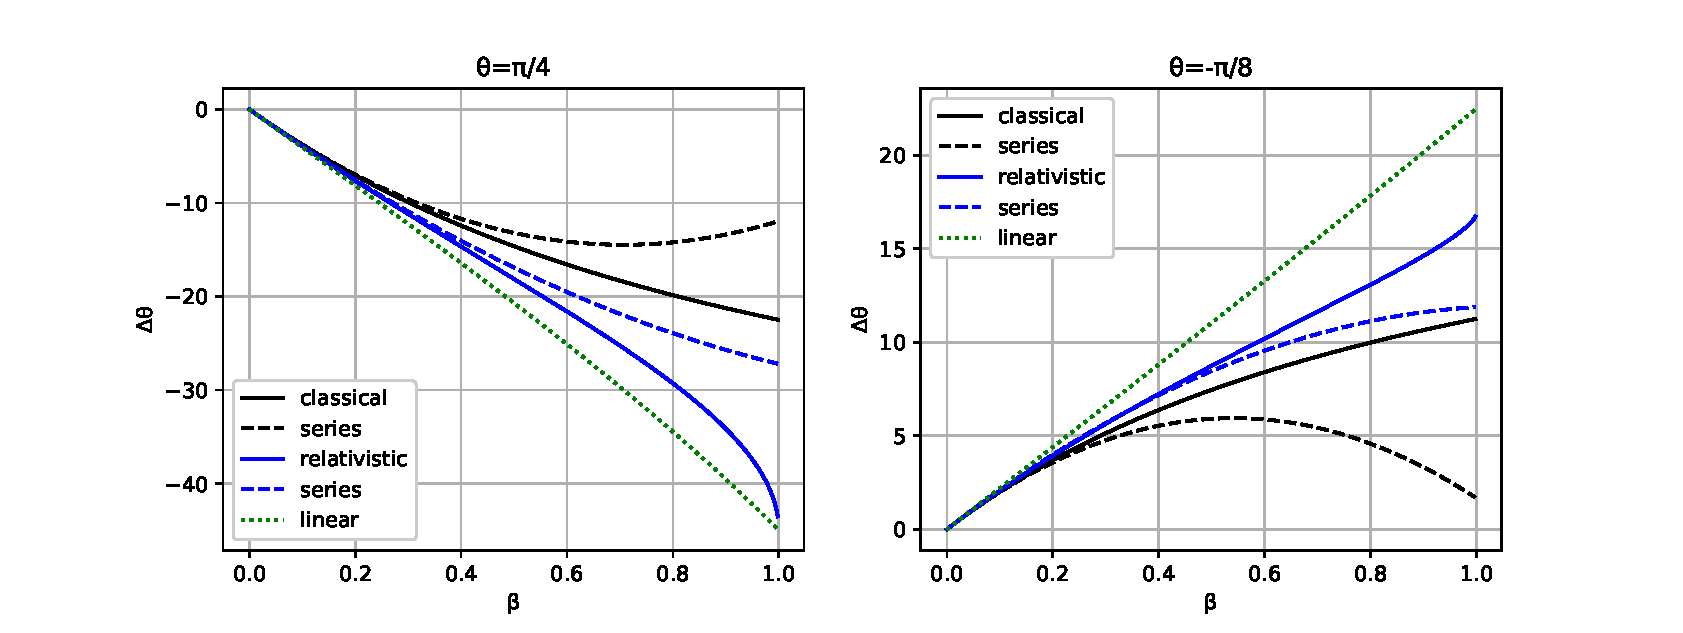
\includegraphics [angle=0, width=1\columnwidth] {fig/aberration_series.eps}
     \caption{\label{fig:series} Linear and quadratic approximation of classical and relativistic aberration.}
  \end {center}
\end {figure} 
\begin {figure}
  \begin {center}
     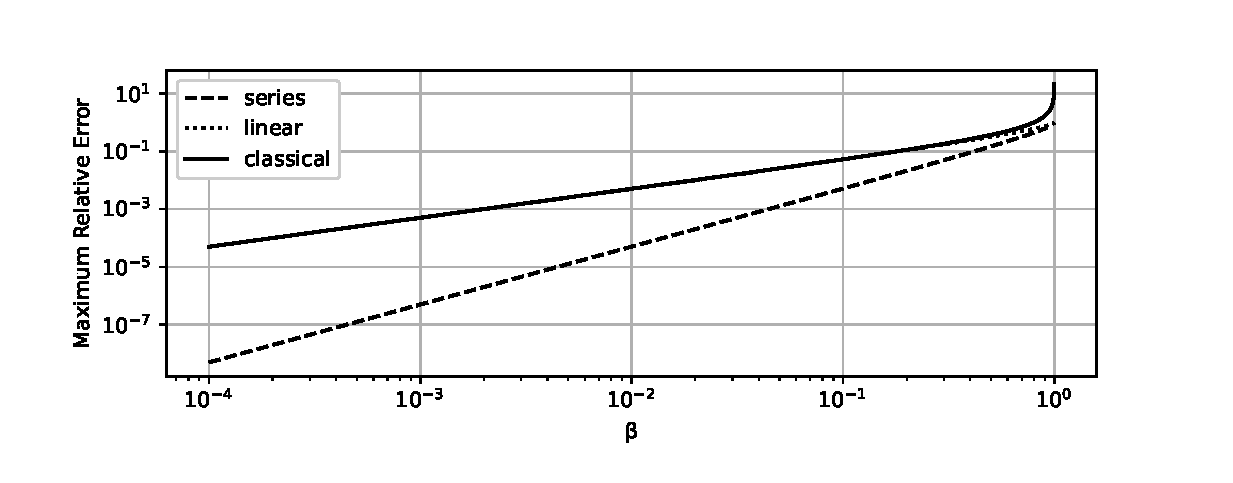
\includegraphics [angle=0, width=1\columnwidth] {fig/aberration_error.eps}
     \caption{\label{fig:error} Maximum aberration error with respect to the exact 
     relativistic formula.}
  \end {center}
\end {figure} 

\subsection{Spherical Coordinates}
We expand uncorrected direction 
\begin {eqnarray}
    \vu p
    = 
    \begin {bmatrix}
        \cos\delta\cos\alpha \\
        \cos\delta\sin\alpha \\
        \sin\delta
    \end {bmatrix},
\end {eqnarray}
where $\delta$ and $\alpha$ are the declination and the right ascension, 
respectively (in appropriate frames). Then, unit vectors along the 
declination and right ascension coordinates can be written 
\begin {eqnarray}
    \vu e_{\delta} =\pdiff{\vu p}{\delta}
    = 
    \begin {bmatrix}
        -\sin\delta\cos\alpha \\
        -\sin\delta\sin\alpha \\
        \cos\delta
    \end {bmatrix},
    \quad
    \vu e_{\alpha} 
    =
    \frac{1}{\cos\delta}\pdiff{\vu p}{\alpha}
    = 
    \begin {bmatrix}
        -\sin\alpha \\
        \cos\alpha \\
        0
    \end {bmatrix}.
\end {eqnarray}
Thus, for small $\vu s - \vu p$, we can approximate 
\begin {eqnarray}
    \Delta\delta &=& (\vu s - \vu p)\cdot\vu e_\delta
    \\
    \cos\delta \Delta\alpha &=& (\vu s - \vu p)\cdot\vu e_\alpha
\end {eqnarray}
For small $v/c$, we can approximate from $(\ref{eq:classical_properdir})$ 
\begin {eqnarray}
    \vu s - \vu p \approx \vc\beta.
\end {eqnarray}
Thereafter, we obtain 
\begin {eqnarray}
    \label{eq:spherical_decl}
    \Delta\delta 
    &=& 
    \vu e_\delta \cdot\vc\beta
    =
    -\beta_x\sin\delta\cos\alpha - \beta_y\sin\delta\sin\alpha + \beta_z\cos\delta
    \\
    \label{eq:spherical_ra}
    \cos\delta\Delta\alpha 
    &=& 
    \vu e_\alpha\cdot\vc\beta 
    = 
    - \beta_x\sin\alpha + \beta_y\cos\alpha.
\end {eqnarray}
\newpage
\section{Stellar Aberration}
\begin {figure}[t]
  \begin {center}
    \begin{tikzpicture}
        \draw[thick] (0, -1) -- (3, -0.5);
        \draw[thick] (0, -1) -- (3, -1.5);
        \draw[thick] (0, -1) -- (2.75, -0.25);
        \draw[thick] (0, -1) -- (2.75, -1.75);
        \draw[thick] (3, -1) ellipse (0.25 and 0.5);
        \draw[thick] (3, -0.425) arc(50:310:0.375 and 0.75);        
        \draw[densely dotted] (0, -1) -- (3, -1);
        \draw[thick, ->] (3, -1) -- (3.5, -1);

        \draw[thick, ->] (0, -1) -- (6, 0.0);
        \draw[thick, ->] (0, -1) -- (5.85, 0.6);
        %\draw (6, 0.0) node{$\bullet$};
        %\draw (5.85, 0.6) node{$\bullet$};
        %\draw (4.75, 0.55) node[rotate=15] {Uncorrected};
        %\draw (4.75, -0.41) node[rotate=9]{Corrected};
        
        \draw[thick, <-] (5, -0.18) arc(-10:60:0.25 and 0.5);
        \draw[thick] (5.5, 0.2) node{$\Delta\theta$};

        \draw (0, -1) node{$\bullet$};
        %\draw (3, -1) node{$\bullet$};
        \draw (4, -1) node{$\vc v$};
        \draw (0, 1) node{$\bullet$};

        \draw[thick] (0, 1) -- (3, 1.75);
        \draw[thick] (0, 1) -- (3, 0.25);
        \draw[thick] (3, 1) ellipse (0.375 and 0.75);
        \draw[thick, ->] (0, 1) -- (6, 2.5);
        \draw[thick, ->] (0, 1) -- (5.85, 3.125);
        %\draw(5.0, 2.0) node[rotate=14] {Uncorrected};
        %\draw (4.5, 2.9) node[rotate=19] {Corrected};
        \draw[thick] (3.125, 1.75) arc(50:310:0.5 and 1);        
        \draw[thick, ->] (0, 1) -- (-2, 1);
        \draw[thick, ->] (5, 2.25) arc(-10:60:0.25 and 0.5);
        \draw[thick] (5.4, 2.65) node{$\Delta\theta$};
        \draw (-2.25, 1) node{$\vc v$};



        %\draw[thick] (0, 1) -- (-3, 0.5);
        %\draw[thick] (0, 1) -- (-3, 1.5);
        %\draw[thick] (0, 1) -- (-2.75, 0.25);
        %\draw[thick] (0, 1) -- (-2.75, 1.75);
        %\draw[thick] (-3, 1) ellipse (0.25 and 0.5);
        %\draw[thick] (-3, 0.425) arc(230:480:0.375 and 0.75);        
        %\draw[densely dotted] (0, 1) -- (-3, 1);
        %\draw[thick, ->] (-3, 1) -- (-3.5, 1);
        %\draw (0, 1) node{$\bullet$};
        %\draw (-3, 1) node{$\bullet$};
        %\draw (-4, 1) node{$\vc v$};

        \draw (0, 0) node{$\bullet$};
        \draw (0, 1.35) node{$\oplus$};
        \draw (0, -0.65) node{$\oplus$};
        \draw (0, 0.35) node{$\sun$};

        \draw[thick] (0,0) ellipse (2 and 1);

        \draw[thick] (9, 0) ellipse (1.5 and 1.5);
        \draw[thick, <-] (10.25, 0) arc(0:180:1.25 and 1.25);
        \draw[densely dotted] (9, 1.5) -- (10.6, 1.5);
        \draw[thick, ->] (10.6, 1.5) -- (11.5, 1.5);
        \draw (9, 1.5) node{$\bullet$};
        \draw (11.75, 1.5) node{$\vc v$};
        \draw[thick, ->] (9, 1.5) -- (12.25, 3.25);
        \draw[thick, ->] (9, 1.5) -- (12.5, 2.5);
        \draw[thick, -] (9, 1.5) -- (10.5, 0.75);
        \draw[thick, -] (9, 1.5) -- (10.6, 1.05);
        \draw[thick, <-] (11.5, 2.25) arc(0:60:0.30 and 0.6);
        \draw (11.8, 2.65) node{$\Delta\theta$};
        %\draw (11.5, 3.2) node[rotate=29] {Uncorrected};
        %\draw (11.5, 2) node[rotate=15] {Corrected};
        \draw[thick] (10.5, 1.5) ellipse (0.375 and 0.75);
        \draw[thick] (10.6, 1.5) ellipse (0.225 and 0.45);

    \end {tikzpicture}
    \caption{\label{fig:aberration_types}Annual aberration correction for a planet 
        orbiting the Sun (left). Diurnal aberration correction for an observer on the 
        surface of a rotating planet (right). The cones depict rotational symmetry in the correction.}
  \end {center}
\end {figure}

\textbf{Stellar aberration} refers to the apparent change in the position 
of a stellar object due to velocity of the observer. For an observer fixed 
to the surface of a rotating planet, the stellar aberration may involve:
\begin {itemize}
    \item \textbf{Annual aberration} resulting from the motion of the planet 
    around the barycenter of the solar system. For Earth, the velocity of 
    $29.79\:$km/s around the barycenter of the solar system amounts to a 
    maximum correction on $20.496$ arcseconds.
    \item \textbf{Diurnal aberration} resulting from the rotation of the 
    planet. At the equator, Earth rotates approximately with the tangential
    velocity of $465$ meters per second, which amounts to a maximum 
    correction of $0.32$ arcseconds.
    \item \textbf{Secular aberration} resulting from the approximately unifrom 
    motion of the solar system around the center of the galaxy. For our 
    solar system, this velocity. is about $220$ km/s and amounts to a 
    maximum correction of 150". However, since the velocity changes very slowly, 
    the effect is included in the catalogued positions and is not corrected.
    \item \textbf{Planetary aberration} resulting from both the motion 
    of the observer and the movement of the observed body. 
\end {itemize}
Aberration can also result from the observer moving w.r.t. 
the surface of the planet. For example, a fighter jet or a missile 
can travel at speeds higher than the rotation speed of Earth. However, 
this effect is likely always small enough to be neglected in technical 
applications.
For a satellite on LEO moving at $8$ km/s w.r.t. inertial frame centered 
on Earth, the maximum aberration is around $5.5$ arcseconds. 

The expressions developed in the previous section apply to all types of 
aberration. 

\subsection{Linear Approximation in Spherical Coordinates}
\subsubsection{Annual Aberration}
For elliptic orbits, the velocity and distance from the center can be 
expressed 
\begin {eqnarray}
    v 
    =
    \sqrt{
        \mu\left(\frac{2}{r} - \frac{1}{a}\right)
    },
    \quad
    r 
    = \frac{a(1-e^2)}{1 + e\cos f}.
\end {eqnarray}
At perihelion and aphelion $f=0$ and $f=180^\circ$, respectively corresponding
to maximum and minimum velocities
\begin {eqnarray}
    v_{max} = \sqrt{
        \frac{\mu}{a}
        \left(
            \frac{1+e}{1-e}
        \right)
    },
    \quad
    v_{min} = \sqrt{
        \frac{\mu}{a}
        \left(
            \frac{1-e}{1+e}
        \right)
    }.
\end {eqnarray}
For Earth's orbit around the Sun, we can substitue 
$\mu = 1.32712440042\cdot 10^{20}\:\textrm{m}^3\textrm{s}^{-2}$, 
$e = 0.01671022$ and $a=1.495980229607128\cdot 10^{11}$ m leading to
\begin {eqnarray}
    v_{max} = 30286.614\:\textrm{m/s},
    \quad
    v_{min} = 29291.058\:\textrm{m/s},
    \quad 
    v_{avg} = 29790.915\:\textrm{m/s}.
\end {eqnarray}
The \textbf{constant of aberration} $\kappa$ is the maximum possible displacement 
of a distant object due to aberration and can be approximated $\kappa\approx v/c$.
Correspondingly, we obtain 
\begin {eqnarray}
    \kappa_{max} = \SI{20.838}{\arcsecond}, 
    \quad
    \kappa_{min} = \SI{20.153}{\arcsecond} , 
    \quad
    \kappa_{avg} = \SI{20.497}{\arcsecond}. 
\end {eqnarray}
To obtain geometric intuition about annual aberration throughout the year, 
consider a circular orbit with zero inclination. That is, 
\begin {eqnarray}
    \vc\beta (t) &=& \beta(\cos\omega t, \sin\omega t, 0).
\end {eqnarray}
Substitution to $(\ref{eq:spherical_decl})$ and $(\ref{eq:spherical_ra})$,
yields 
\begin {eqnarray}
    \Delta\delta &=& 
    -\beta \sin\delta\cos\alpha \cos\omega t
    -\beta \sin\delta\sin\alpha \sin\omega t
    \\
    \cos\delta\Delta\alpha &=& 
    -\beta \sin\alpha \cos\omega t
    +\beta \cos\alpha \sin\omega t.
\end {eqnarray}
Suppose $\alpha=0$. Then, the above simplifies to 
\begin {eqnarray}
    \Delta\delta &=& 
    -\beta \sin\delta\cos\omega t,
    \\
    \cos\delta\Delta\alpha &=& 
    \beta\sin\omega t.
\end {eqnarray}
That is, annual aberration will lead to a displacement shaped like an ellipse
with a period of one orbit (see Figure \ref{fig:aberration_ellipse}).

\begin {figure}[t]
  \begin {center}
    \begin{tikzpicture}
        \draw[thick] (-2, 0) -- (-2, 1.5);
        \draw[thick] (0, 0) -- (0, 1.5);
        \draw[thick] (0, 0) -- (2.5, 0);
        \draw[thick] (0, -1) -- (2.5, -1);
        \draw[thick, <->] (-2, 1.25) -- (0, 1.25);
        \draw[thick, <->] (2.25, -1) -- (2.25, 0);
        \draw[thick, ->] (0, 0) -- (2.75, 0);
        \draw[thick, ->] (0, 0) -- (0, 1.75);
        \draw (0, -1) node{$\bullet$};
        \draw (0, 0) node{$\bullet$};
        \draw (-2, 0) node{$\bullet$};
        %\draw (0, -1.3) node{$\earth$};
        %\draw (0, -0.3) node{$\sun$};

        \draw[thick] (0,0) ellipse (2 and 1);
        \draw (-1, 1.55) node{$\beta$};
        \draw (2.5, -0.5) node{$\:\:\quad\quad \beta\sin\delta$};
        \draw (-0.5, -0.25) node{$(\alpha, \delta)$};

        \draw (2.75, 0.35) node{$\:\:\Delta\alpha\cos\delta$};
        \draw (0.25, 1.5) node{$\:\:\Delta\delta$};
    \end {tikzpicture}
    \caption{\label{fig:aberration_ellipse}Elliptical shape of abberation correction w.r.t.
            the uncorrected position.}
  \end {center}
\end {figure}
\subsubsection{Diurnal Aberration}
The velocity of the observer on the surface of Earth can be written
\begin {eqnarray}
    v = \omega(R + h)\cos\phi,
\end {eqnarray}
where $R, h$ and $\phi$ are the radius of Earth, altitude of the observer 
above the surface of Earth and the latitude. Consequently, the aberration 
can be approximated
\begin {eqnarray}
    \Delta\theta \approx \beta \approx \frac{\omega(R + h)}{c}\cos\phi.
\end {eqnarray}
Substitution of $R= 6371\:$km, $\omega = 2\pi/86164.0905$ s yields at the 
equator
\begin {eqnarray}
    \Delta\theta \approx -\SI{0.3196}{\arcsecond}.
\end {eqnarray}
The velocity is always approximately towards the east corresponding to the 
x-axis in the ENU frame. That is, substituting $\vc\beta=\beta\vu x$ to 
$(\ref{eq:spherical_decl})$ and $(\ref{eq:spherical_ra})$, yields 
\begin {eqnarray}
    \Delta\delta &=& - \beta\sin\delta\cos\alpha 
    \\
    \cos\delta\Delta\alpha &=& - \beta\sin\alpha.
\end {eqnarray}
The notation above is misleading in the sense $\delta$ and $\alpha$ do not 
refer to declination and right ascension. To obtain an expression in terms 
of elevation and azimuth, substitute for $a = \delta$ and 
$\alpha = 90^\circ - \phi$ to obtain 
\begin {eqnarray}
    \Delta a &=& -\beta\sin a\sin\phi, \\
    \cos a\Delta\phi &=& \beta\cos\phi.
\end {eqnarray}
For $\phi = 90^\circ$ (east), we obtain $\Delta a = -\beta\sin a$ and for 
$a = 0$, we obtain $\Delta\phi = \beta\cos\phi = -\beta\sin (\phi - 90^\circ)$, 
which is consistent with $(\ref{eq:relativistic_series})$.

\subsection{Planetary Aberration and Light-Time}
The travel time of light between target and the observer is called 
\textbf{light-time} and denoted $\tau$. When the direction to target 
changes significantly during light-time, this requires a correction. 
The relative apparent position to target can be expressed 
\begin {eqnarray}
    \vc p(t) = \vc u_B(t - \tau) - \vc E_B(t),
\end {eqnarray}
where $\vc u_B$ and $\vc E_B$ are the barycentric positions of the 
target and the observer. Application of $(\ref{eq:classical_properdir})$ 
yields 
\begin {eqnarray}
    \vc s(t) &=& \vc p(t) + \beta|\vc p|
    \\
    &=& 
    \vc u_B(t - \tau) - \vc E_B(t) + \frac{|\vc p|}{c}\dot{\vc E_B}(t)
    \\
    &=& 
    \vc u_B(t - \tau) - \vc E_B(t) + \tau\dot{\vc E_B}(t)
    \\
    &\approx& 
    \vc u_B(t - \tau) - \vc E_B(t - \tau).
\end {eqnarray}
That is, correcting for planetary aberration at $t$ with classical approximation 
$(\ref{eq:classical_properdir})$ is equivalent to the computation the uncorrected 
direction to target at $t-\tau$. Note that this does not take into account 
the diurnal aberration.

\subsection{Practical Computation}
The positions of stars are typically catalogued w.r.t. the Solar System 
Barycenter (SSB) so that secular aberration is already included in the 
catalogued positions. Thus, to compute the aberration correction for an 
observer, we need to compute the velcoity vector of the observer w.r.t. 
the SSB. For an observer on Earth, this velocity is the sum of the 
orbital velocity of the Earth around the SSB and the rotational velocity 
of the topocentric position of the observer around the geocenter (GEO) of 
Earth. Thereafter, $(\ref{eq:classical_properdir})$ and 
$(\ref{eq:properdir2})$ can be applied in any topocentric frame centered 
on the observer position.

\subsubsection{Transformations Between Frames}
Let us denote the position and velocity coordinate vector for target 
$C$ in frame with orientation $A$ and origin $B$ with $\vc r_{C(A)}^B$
and $\vc v_{C(A)}^B$. Omission of $C$, $A$ or $B$ in an expression 
signifies that the expression applies for all targets, orientations or 
origins, respectively. Then, if $R_A^a$ is the rotation matrix from
orientation a to A, we can write 
\begin {eqnarray}
    \label{eq:posrotation}
    \vc r_{(A)} = R_A^a\vc r_{(a)}
    \quad\Leftrightarrow\quad
    \vc r_{C(A)}^B = R_A^a\vc r_{C(a)}^B
    \quad 
    \forall B, C.
\end {eqnarray}
Similarly, for any two origins B and b 
\begin {eqnarray}
    \vc r^B = \vc r^b - \vc r^b_B 
    \quad\Leftrightarrow\quad
    \vc r_{C(A)}^B = \vc r_{C(A)}^b - \vc r_{B(A)}^b 
    \quad 
    \forall A, C.
\end {eqnarray}
The equation $(\ref{eq:posrotation})$ does not apply to velocity vectors
unless the rotation matrix is constant w.r.t. time. More generally, we can 
expand  
\begin {eqnarray}
    \vc v_{(A)}
    =
    \diff{}{t}\vc r_{(A)}
    = 
    \diff{}{t}\left(
        R_A^a\vc r_{(a)}
    \right)
    =
    \dot{R_A^a}\vc r_{(a)}
    +
    R_A^a
    \vc v_{(a)},
\end {eqnarray}
where the $\dot R_A^a\vc r_{(a)}$ corresponds to velocity component from 
the rotation of $\vc r_{(a)}$ w.r.t. the origin.

\subsubsection{Expansion of the Observer Velocity}
The position and velocity vectors w.r.t. origins at the GEO and the SSB
can be related by
\begin {eqnarray}
    \vc r^{GEO} &=& \vc r^{SSB} - \vc r_{GEO}^{SSB}, \\
    \vc v^{GEO} &=& \vc v^{SSB} - \vc v_{GEO}^{SSB},
\end {eqnarray}
where $\vc v_{GEO}^{SSB}$ is the orbital velocity of the geocenter w.r.t. 
the SSB. The rotation of the Earth can be expressed via the coordinate 
transform between inertial True-of-Date (ToD) and Pseudo-Earth-Fixed (PEF) 
frames 
\begin {eqnarray}
    \vc r_{(PEF)}^{GEO} 
    &=&
    R_{PEF}^{TOD} \vc r_{(TOD)}^{GEO}
    \quad : \quad 
    R_{PEF}^{TOD}
    =
    \begin {bmatrix}
        \cos GAST & \sin GAST & 0 \\
        -\sin GAST & \cos GAST & 0 \\
        0 & 0 & 1
    \end {bmatrix},
    \\
    \vc r_{(TOD)}^{GEO} 
    &=&
    R_{TOD}^{PEF} \vc r_{(PEF)}^{GEO}
    \quad : \quad 
    R_{TOD}^{PEF}
    =
    \begin {bmatrix}
        \cos GAST & -\sin GAST & 0 \\
        \sin GAST & \cos GAST & 0 \\
        0 & 0 & 1
    \end {bmatrix}.
\end {eqnarray}
where GAST is the Greenwich Apparent Sidereal Time. The corresponding velocities
can be expanded 
\begin {eqnarray}
    \vc v_{(PEF)}^{GEO}
    &=&
    R_{PEF}^{TOD}\vc v_{(TOD)}^{GEO}
    +
    {{\dot R}_{PEF}^{TOD}}\vc r_{(TOD)}^{GEO},
    \\
    \vc v_{(TOD)}^{GEO}
    &=&
    R_{TOD}^{PEF}\vc v_{(PEF)}^{GEO}
    +
    {{\dot R}_{TOD}^{PEF}}\vc r_{(PEF)}^{GEO},
\end {eqnarray}
where 
\begin {eqnarray}
    {{\dot R}_{PEF}^{TOD}} 
    &=&
    \diff{GAST}{t} 
    \begin {bmatrix}
        -\sin GAST & \cos GAST & 0 \\
        -\cos GAST & -\sin GAST & 0 \\
        0 & 0 & 0
    \end {bmatrix}
    \\
    {{\dot R}_{TOD}^{PEF}} 
    &=&
    \diff{GAST}{t} 
    \begin {bmatrix}
        -\sin GAST & -\cos GAST & 0 \\
        \cos GAST & -\sin GAST & 0 \\
        0 & 0 & 0
    \end {bmatrix}.
\end {eqnarray}
For computation of diurnal aberration amounting to less than $0.32$ arcseconds, 
we can approximate the time derivative of GAST using the length of a sidereal 
day
\begin {eqnarray}
    \diff{GAST}{t}
    \approx 
    \frac{2\pi\:\textrm{rad}}{86164.0905\:s}
    \approx 7.2921159\cdot 10^{-5} \textrm{rad/s}
    \approx 15.04107^\circ /h.
\end {eqnarray}
The velocity of the observer w.r.t. the SSB can be expressed 
\begin {eqnarray}
    \vc v_{(ECL)}^{SSB} 
    &=& 
    \vc v_{GEO,(ECL)}^{SSB} + R_{ECL}^{TOD}\vc v_{(TOD)}^{GEO} 
    \\
    &=& 
    \vc v_{GEO,(ECL)}^{SSB} + R_{ECL}^{TOD}
    \left(
    R_{TOD}^{PEF}\vc v_{(PEF)}^{GEO}
    +
    {{\dot R}_{TOD}^{PEF}}\vc r_{(PEF)}^{GEO}
    \right).
\end {eqnarray}
The position of the observer 
$\vc r_{(PEF)}^{GEO} = R_{PEF}^{EFI}\vc r_{(EFI)}^{GEO}$, where 
$\vc r_{(EFI)}^{GEO}$ can obtained from geodetic position on WGS84.
For an observer that is stationary w.r.t. surface of Earth 
$\vc v_{(PEF)}^{GEO} = \vc 0$.

Aberration corrections $(\ref{eq:classical_properdir})$ and 
$(\ref{eq:properdir2})$ can be applied in the ecliptic frame centered 
on the SSB or the topocentric ENU frame of the observer. Application in an 
ENU frame requires rotation 
\begin {eqnarray}
    R^{ECL}_{ENU}\vc v_{(ECL)}^{SSB} 
    &=& 
    R^{ECL}_{ENU}\vc v_{GEO,(ECL)}^{SSB} + R_{ENU}^{TOD}
    \left(
    R_{TOD}^{PEF}\vc v_{(PEF)}^{GEO}
    +
    {{\dot R}_{TOD}^{PEF}}\vc r_{(PEF)}^{GEO}
    \right).
\end {eqnarray}
Note that since the aberration relates to the velocity difference between 
the observer and the SSB in an inertial frame, it is not appropriate to 
transfer the velocity of SSB to a topocentric frame, where it would rotate 
around the observer location at very high speed.


\newpage
\section{Doppler Effect}
\subsection{Classical and Relativistic Doppler Effect}
\begin {figure}[t]
  \begin {center}
    \begin{tikzpicture}
        \clip (-0.5, -1.5) rectangle (9, 1.5);
\draw[color=gray!50] (7-5.5, 0.5) circle (3.5);
\draw[color=gray!50] (7-5.375, 0.5) circle (3.25);
\draw[color=gray!50] (7-5.25, 0.5) circle (3.0);
\draw[color=gray!50] (7-5.125, 0.5) circle (2.75);
\draw[color=gray!50] (7-5.0, 0.5) circle (2.5);
\draw[color=gray!50] (7-4.875, 0.5) circle (2.25);
\draw[color=gray!50] (7-4.75, 0.5) circle (2.0);
\draw[color=gray!50] (7-4.625, 0.5) circle (1.75);
\draw[color=gray!50] (7-4.5, 0.5) circle (1.5);
\draw[color=gray!50] (7-4.375, 0.5) circle (1.25);
\draw[color=gray!50] (7-4.25, 0.5) circle (1.0);
\draw[color=gray!50] (7-4.125, 0.5) circle (0.75);
\draw[color=gray!50] (7-4.0, 0.5) circle (0.5);
\draw[color=gray!50] (7-3.875, 0.5) circle (0.25);

        \draw[thick] (0, 0) -- (3, 0);
        \draw[thick] (0, 1) -- (3, 1);
        \draw[thick] (0, 0) -- (0, 1);
        \draw[thick] (3, 0) -- (3, 1);
        \draw[thick, ->] (3, 0.5) -- (6, 0.5);
        \draw[thick] (3, 0.5) -- (5, -0.5);
        \draw[thick] (1.5, 0.5) node{Emitter ($S'$)};
        \draw[thick] (4.5, 0.8) node{$v$};
        \draw[thick] (3.7, 0.14) arc(-45:0:0.5 and 0.5);
        \draw[thick] (4.1, 0.3) node{$\theta$};
        \draw[thick] (5.5, -0.7) ellipse (0.5 and 0.5);
        \fill[black] (5.25, -0.55) ellipse (0.10 and 0.15);
        \draw[thick] (5.25, -0.55) ellipse (0.175 and 0.25);
        \draw[thick] (7.5, -0.5) node{Observer ($S$)};
   \end {tikzpicture}
    \caption{\label{fig:doppler_effect} Geometry associated to Doppler Effect.}
  \end {center}
\end {figure}


Consider a light source fixed to an inertial frame $S'$ moving with velocity $v$ 
w.r.t. an observer fixed to an inertial frame $S$ (see Figure 
\ref{fig:doppler_effect}). Suppose that the direction of movement makes the angle 
$\theta$ w.r.t. direction to the observer. Let $\vc v = v\vu x$ and represent the 
wavefront towards the observer with phase angle
\begin {eqnarray}
    \phi(\vc x, t) = A\cos(\vc k\cdot\vc x - \omega t),
\end {eqnarray}
where the wave vector satisfies 
\begin {eqnarray}
    \vc k = k\cos\theta\:\vu x + k\sin\theta\:\vu y.
\end {eqnarray}
Substitution of $kx-\omega t = 0$ yields in vacuum $x = \omega t / k = ct$ and 
$k = \omega/c$.

The phase angle $\phi$ in the frames $S$ and $S'$ can be related by the Galilean
transformation
\begin {eqnarray}
    t &=& t' \\
    x &=& x' + vt \\
    y &=& y' \\
    z &=& z'
\end {eqnarray}
with the expansion 
\begin {eqnarray}
    \vc k\cdot\vc x - \omega t
    &=&
    kx \cos\theta + ky \sin\theta - \omega t 
    \\
    &=& 
    k(x' + vt) \cos\theta + ky \sin\theta - \omega t 
    \\
    &=& 
    kx'\cos\theta + ky'\sin\theta -\omega(1 -\beta\cos\theta)
    \\
    &=& 
    \vc k'\cdot\vc x' - \omega' t
\end {eqnarray}
Thus, we obtain the expression for \textbf{classical Doppler Effect}
\begin {eqnarray}
    \boxed{
        \quad
        \omega = \frac{\omega'}{1 - \beta\cos\theta},
        \quad
        \vc k' = \vc k.
        \quad
    }
\end {eqnarray}
In the relativistic case, we replace the Galilean transformation with the Lorentz 
transformation 
\begin {eqnarray}
    t &=& \gamma(t' + \beta x'/c) \\
    x &=& \gamma(x' + vt) \\
    y &=& y' \\
    z &=& z'.
\end {eqnarray}
Now we can expand 
\begin {eqnarray}
    \vc k\cdot\vc x - \omega t 
    &=& 
    k\gamma(x' + vt')\cos\theta + ky\sin\theta  - \omega\gamma(t' + \beta x'/c)
    \\
    &=& 
    \gamma (k\cos\theta - \omega\beta/c)x' 
    + 
    ky\sin\theta 
    - 
    \gamma(\omega - kv\cos\theta)) t'
    \\
    &=& 
    \gamma k (\cos\theta - \beta)x'
    +
    ky'\sin\theta 
    -
    \gamma\omega(1 - \beta\cos\theta)t'
    \\
    &=& 
    \vc k'\cdot\vc x' - \omega' t' 
\end {eqnarray}
and obtain the expression for \textbf{relativistic Doppler Effect}
\begin {eqnarray}
    \label{eq:doppler_relativistic}
    \boxed{
        \quad
        \omega = \frac{\omega'}{\gamma(1 - \beta\cos\theta)},
        \quad
        \vc k' = \gamma k(\cos\theta - \beta)\vu x 
        +
        k\sin\theta\vu y.
        \quad
    }
\end {eqnarray}
The transformation of the wave vector corresponds to the relativistic aberration 
correction. 

\subsection{Interpretation}
\subsubsection{Longitudal Doppler Effect}
The special cases relating to longitudal motion are depicted in Figure \ref{fig:redshift_blueshift}.
When $\theta = 180^\circ$ and $\theta = 0^\circ$, we can expand 
\begin {eqnarray}
    \frac{\omega}{\omega'}
    &=&
    \frac{1}{\gamma(1 + \beta)}
    =
    \frac{\sqrt{(1 + \beta)(1 - \beta)}}{1 + \beta}
    = 
    \sqrt{\frac{1 - \beta}{1 + \beta}} \leq 1
    \\
    \frac{\omega}{\omega'}
    &=&
    \frac{1}{\gamma(1 - \beta)}
    =
    \frac{\sqrt{(1 + \beta)(1 - \beta)}}{1 - \beta}
    = 
    \sqrt{\frac{1 + \beta}{1 - \beta}} \geq 1
\end {eqnarray}
respectively. 
\begin {figure}[h]
  \begin {center}
    \begin{tikzpicture}
        \draw[thick] (0, -2) -- (3, -2);
        \draw[thick] (0, -1) -- (3, -1);
        \draw[thick] (0, -2) -- (0, -1);
        \draw[thick] (3, -2) -- (3, -1);
        \draw[thick, ->] (3, -1.5) -- (5, -1.5);
        \draw[thick] (1.5, -1.5) node{Emitter ($S'$)};
        \draw[thick] (4.5, -1.2) node{$v$};
        \draw[thick] (4.1, -1.7) node{$\theta=0$};
        \draw[thick] (5.5, -1.5) ellipse (0.5 and 0.5);
        \fill[black] (5.25, -1.5) ellipse (0.10 and 0.15);
        \draw[thick] (5.25, -1.5) ellipse (0.175 and 0.25);
        \draw[thick] (7.5, -1.5) node{Observer ($S$)};

        \draw[thick] (0, 0) -- (3, 0);
        \draw[thick] (0, 1) -- (3, 1);
        \draw[thick] (0, 0) -- (0, 1);
        \draw[thick] (3, 0) -- (3, 1);
        \draw[thick, dotted] (0, 0.5) -- (-2, 0.5);
        \draw[thick] (4.5, 0.8) node{$v$};
        \draw[thick, ->] (3, 0.5) -- (5, 0.5);

        \draw[thick] (1.5, 0.5) node{Emitter ($S'$)};
        \draw[thick] (-0.9, 0.3) node{$\theta=180^\circ$};
        \draw[thick] (-2.5, 0.5) ellipse (0.5 and 0.5);
        \fill[black] (-2.25, 0.5) ellipse (0.10 and 0.15);
        \draw[thick] (-2.25, 0.5) ellipse (0.175 and 0.25);
        \draw[thick] (-4.5, 0.5) node{Observer ($S$)};
        \end {tikzpicture}
    \caption{\label{fig:redshift_blueshift} Geometry associated to maximal 
             redshift (top) and maximal blueshift (below).}
  \end {center}
\end {figure}
\subsubsection{Transverse Doppler Effect}
With transverse motion, it is necessary to take into account the influence of
aberration: The meaning of the direction of movement being at right angles to 
the vector between the observer and the source is dependent on the frame. 
Superficial analysis not taking aberration into account might suggest that a 
planet orbiting a star a perfectly circular orbit would experience Doppler 
redshift but in fact it will experience blueshift.

Substitution of $\theta = \pi/2$ to $(\ref{eq:doppler_relativistic})$ yields 
expression for transverse motion in $S$
\begin {eqnarray}
    \omega = \frac{\omega'}{\gamma} < \omega'
\end {eqnarray}
However, substitution of $\theta' = \pi/2$ yields $\beta = \cos\theta$ and 
an expression for transverse motion in $S'$
\begin {eqnarray}
    \omega = \frac{\omega'}{\gamma(1 - \beta^2)} = \gamma\omega' > \omega'.
\end {eqnarray}
That is, transverse motion from the viewpoint of the observer leads to a 
redshift and transverse motion from the viewpoint of the source leads to 
a blueshift. A planet orbiting a star on a circular orbit will experience 
Doppler blueshift of the starlight and a imaging satellite orbiting a planet 
will experience (Doppler) redshift (see Figure \ref{fig:doppler_transverse}).

\begin {figure}[t]
  \begin {center}
    \begin{tikzpicture}
        \draw (7, 0) node{$\bullet$};
        \draw (7, 0.35) node{$\sun$};
        %\draw[thick] (0,0) circle (2);

        \draw[thick] (9.0, 0) ellipse (0.5 and 0.5);
        \fill[black] (8.75, 0) ellipse (0.10 and 0.15);
        \draw[thick] (8.75, 0) ellipse (0.175 and 0.25);
        \draw[thick] (10.75, 0) node{Observer ($S$)};
        \draw[thick] (7, -0.5) node{Source ($S'$)};
        \draw[thick] (9,0.5) arc (15:345:2);
        \draw[thick, ->] (9, 0.5) -- (9, 2);
        \draw[thick] (9.2, 1) node{$v$};

        \draw[thick] (0,0) circle (2);
        \draw[thick] (0.0, 0) ellipse (0.5 and 0.5);
        \fill[black] (0.25, 0) ellipse (0.10 and 0.15);
        \draw[thick] (0.25, 0) ellipse (0.175 and 0.25);
        \draw[thick] (2, 0) node{$\bullet$};
        \draw (1.65, 0) node{$\sun$};
        \draw[thick, ->] (2, 0.0) -- (2, 2);
        \draw[thick] (2.2, 1) node{$v$};
        \draw[thick] (0.0, -0.75) node{Observer ($S$)};
        \draw[thick] (3.25, 0.0) node{Source ($S'$)};

    \end {tikzpicture}
    \caption{\label{fig:doppler_transverse} Two examples of transverse motion:
    Transverse motion in $S$ resulting in redshift (left) and transverse motion 
    in $S'$ resulting in blueshift (right).}
  \end {center}
\end {figure}


\subsubsection{Boundary Between Redshift and Blueshift}
As shown previously, maximum blueshift and redshift are obtained at angles 
$\theta=0^\circ$ and $\theta=180^\circ$, respectively. The boundary w.r.t. 
values $\theta$ between redshift and blueshift occurs when $\omega=\omega'$
or equivalently 
\begin {eqnarray}
    \gamma(1 - \beta\cos\theta) = 1
    &\Leftrightarrow&
    \cos\theta = \frac{1}{\beta}\left(1 - \frac{1}{\gamma}\right).
\end {eqnarray}
The limit is depicted in Figure \ref{fig:doppler_limits}. When $\beta$ 
becomes larger, the region of blueshift gets smaller and converges to a 
dot when $\beta\to 1$. 
\begin {figure}
  \begin {center}
     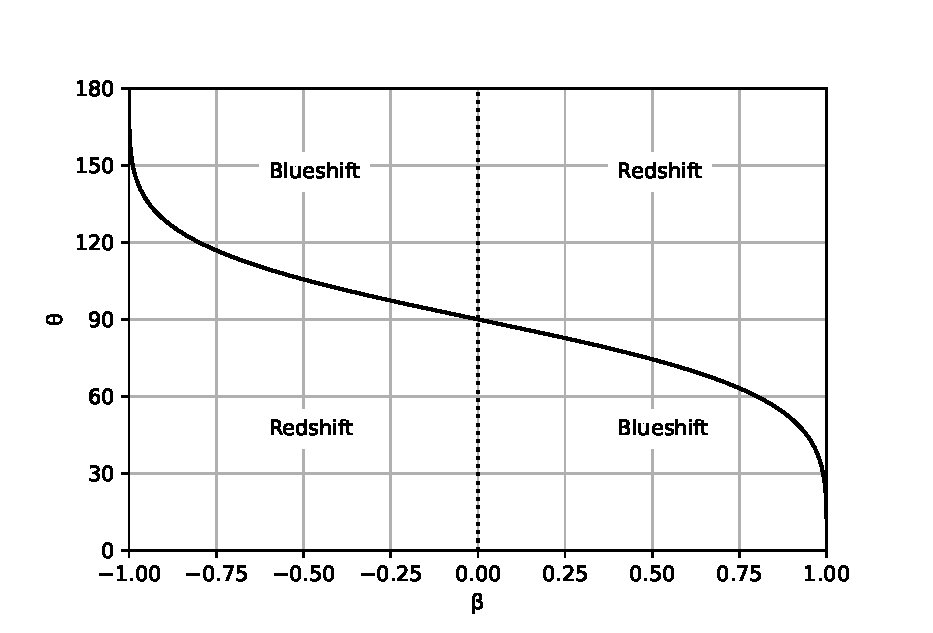
\includegraphics [angle=0, width=0.8\columnwidth] {fig/doppler_limits.eps}
     \caption{\label{fig:doppler_limits} Limit angle between redshift and blueshift.
     For positive and negative $\beta$, the value is the lower and upper limit, respectively 
     of the blueshift for $\theta$.}
  \end {center}
\end {figure} 

\newpage
\section{Perception and Spectrum}
\subsection{Visual Perception}
\subsubsection{Human Vision and LMS Color Space}
Human vision is limited to the wavelength range between 380 and 700 nm. The 
perception of color is based on three classes of cone cells on the retina.
Each type of cone cell has different \textbf{spectral sensitivity}. That is,
they are sensitive to different ranges of wavelengths. We can refer to the 
three classes according to their peak wavelength as long (L), medium (M) and 
short (S) with peaks at 560, 530 and 420 nm, respectively.

Let $S(\lambda)$ be the \textbf{spectral power distribution} 
($\textrm{W}/\textrm{m}^2/\textrm{nm}$) of the light received by the eye.
If $\overline L(\lambda), \overline M(\lambda), \overline S(\lambda)$ are 
cone response functions 
\begin {eqnarray}
    L &=& \int_0^\infty S(\lambda)\overline L(\lambda)\:d\lambda 
    \\
    M &=& \int_0^\infty S(\lambda)\overline M(\lambda)\:d\lambda 
    \\
    S &=& \int_0^\infty S(\lambda)\overline S(\lambda)\:d\lambda,
\end {eqnarray}
they are called \textbf{Color Matching Functions (CMFs)} for the 
\textbf{LMS Color Space}. The cone response functions are normalized 
so that their maxima are equal to unity (see Figure \ref{fig:lms_colormatch}).
The triplets $(L, M, S)$ obtained above are called the \textbf{tristimulus 
values}. Two different spectra resulting in the same tristimulus values are 
called \textbf{metamers}.

\begin {figure}
  \begin {center}
     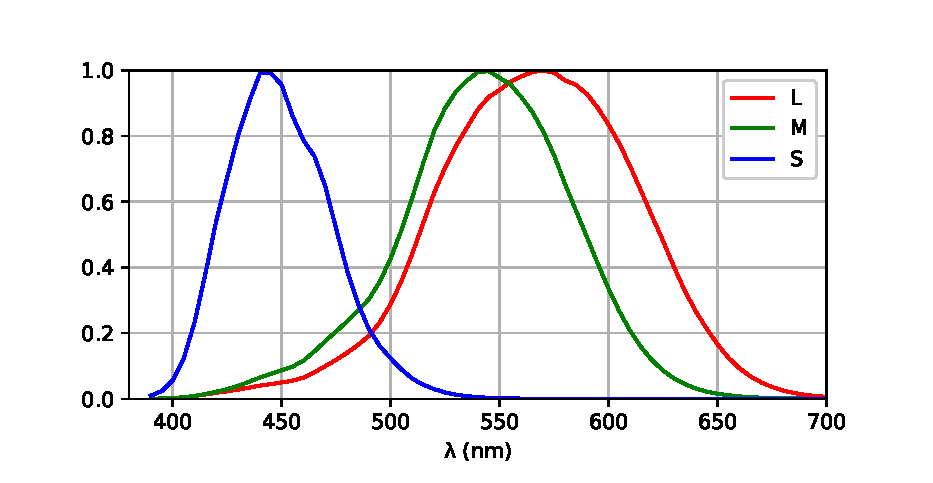
\includegraphics [angle=0, width=0.8\columnwidth] {fig/lms_colormatch.eps}
     \caption{\label{fig:lms_colormatch} LMS color-matching functions
     $\overline L(\lambda), \overline M(\lambda), \overline S(\lambda)$.}
  \end {center}
\end {figure} 


% TBA: https://en.wikipedia.org/wiki/CIE_1931_color_space
% TBA: https://en.wikipedia.org/wiki/LMS_color_space
% TBA: https://www.fourmilab.ch/documents/specrend


\subsubsection{CIE 1931 Color Spaces and sRGB Encoding}
We wish to convert spectrum to 8-bit sRGB values that can be rendered on 
computer displays. This can be achieved by the use of CIE XYZ color-matching
functions and then performing a conversion to SRGB and subsequent 
quantization.
\begin {figure}
  \begin {center}
     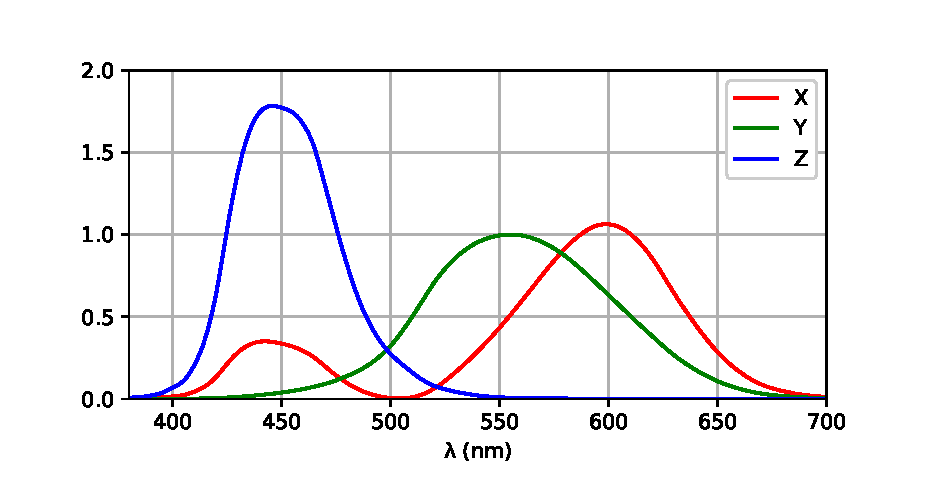
\includegraphics [angle=0, width=0.8\columnwidth] {fig/cie_XYZ.eps}
     \caption{\label{fig:cie_XYZ_colormatch} The CIE XYZ color-matching functions
     $\overline X(\lambda), \overline Y(\lambda), \overline Z(\lambda)$.}
  \end {center}
\end {figure}
The XYZ color-matching functions are shown in Figure \ref{fig:cie_XYZ_colormatch}
and the corresponding tristimulus values are obtained via the inner products 
\begin {eqnarray}
    X &=& \int_0^\infty S(\lambda)\overline X(\lambda)\:d\lambda 
    \\
    Y &=& \int_0^\infty S(\lambda)\overline Y(\lambda)\:d\lambda 
    \\
    Z &=& \int_0^\infty S(\lambda)\overline Z(\lambda)\:d\lambda.
\end {eqnarray}
%\begin {eqnarray}
%    x &=& X / (X + Y + Z), \\
%    y &=& Y / (X + Y + Z), \\
%    z &=& Z / (X + Y + Z)
%\end {eqnarray}
%\begin {eqnarray}
%    z = 1 - (x + y).
%\end {eqnarray}
%\subsubsection{RGB Values and 8-Bit Encoding}
Then, linear sRGB values between in the interval $[0, 1]$ can be obtained via
the matrix product
\begin {eqnarray}
    \label{eq:sRGB}
    \begin {bmatrix}
        R_{sRGB} \\
        G_{sRGB} \\
        B_{sRGB} 
    \end {bmatrix}
    =
    \begin {bmatrix}
        3.2406255 & -1.5372080 & -0.4986286 \\
        -0.9689307 & 1.8757561 & 0.0415175 \\
        0.0557101 & -0.2040211 & 1.0569959         
    \end {bmatrix}
    \begin {bmatrix}
        X \\
        Y \\
        Z 
    \end {bmatrix}
\end {eqnarray}
and clipping values below $0$ and above $1$ to $0$ and $1$, respectively.
Before quantization, a "gamma" transfer function is applied
\begin {eqnarray}
    \label{eq:sRGB2}
    C_{sRGB}' &=& 
    \left\{
    \begin {array}{ll}
        %-1.055(-C_{sRGB})^{(1/2.4)} + 0.55, & C_{sRGB} < -0.0031308 \\
        12.92\:C_{sRGB}, & C_{sRGB} \leq 0.0031308 \\
        1.055(C_{sRGB})^{(1/2.4)} - 0.055, & C_{sRGB} > 0.0031308
    \end {array}
    \right.
\end {eqnarray}
where $C \in \{R, G, B\}$. Finally, the 8-bit quantized values are obtained via
\begin {eqnarray}
    \begin {bmatrix}
        R_{sRGB(8)} \\
        G_{sRGB(8)} \\
        B_{sRGB(8)}
    \end {bmatrix}
    =
    \textrm{round}
    \left(
        255
        \begin {bmatrix}
            R_{sRGB}' \\
            G_{sRGB}' \\
            B_{sRGB}' 
        \end {bmatrix}
    \right)
\end {eqnarray}


%\begin {eqnarray}
%    \begin {bmatrix}
%        Y_{sYCC}' \\
%        Cb_{sYCC}' \\
%        Cr_{sYCC}' 
%    \end {bmatrix}
%    =
%    \begin {bmatrix}
%        0.2990 & 0.5870 & 0.1440 \\
%        -0.1687 & -0.3313 & 0.5000 \\
%        0.5000 & -0.4187 & -0.0813
%    \end {bmatrix}
%    \begin {bmatrix}
%        R_{sRGB}' \\
%        G_{sRGB}' \\
%        B_{sRGB}' 
%    \end {bmatrix}
%\end {eqnarray}
%\begin {eqnarray}
%    Y_{sYCC(8)} &=& \textrm{round}
%    \left[
%        255\:Y_{sYCC}' 
%    \right]
%    \\
%    Cb_{sYCC(8)} &=& \textrm{round}
%    \left[
%        (255\:Cb_{sYCC}') + 128 
%    \right]
%    \\
%    Cr_{sYCC(8)} &=& \textrm{round}
%    \left[
%        (255\:Cr_{sYCC}') + 128 
%    \right]
%\end {eqnarray}

\subsubsection{Example: Visible Wavelength Range}
To compute sRGB values corresponding to the visible wavelength range, select
for each wavelength $\lambda'$
\begin {eqnarray}
    \label{eq:diracwavel}
    S(\lambda) := \frac{1}{2}\delta(\lambda - \lambda'),
\end {eqnarray}
where $\delta$ is the Dirac delta function. The factor is used to avoid 
saturation in cases where the linear sRGB values become larger than 1. Then, 
\begin {eqnarray}
    X &=& 
    \frac{1}{2}
    \int_0^\infty \delta(\lambda - \lambda')\overline X(\lambda)\:d\lambda 
    =
    \frac{1}{2}\overline X(\lambda'),
    \\
    Y &=& 
    \frac{1}{2}\int_0^\infty \delta(\lambda - \lambda')\overline Y(\lambda)\:d\lambda 
    =
    \frac{1}{2}\overline Y(\lambda'),
    \\
    Z &=& 
    \frac{1}{2}\int_0^\infty \delta(\lambda - \lambda')\overline Z(\lambda)\:d\lambda
    =
    \frac{1}{2}\overline Z(\lambda'),
\end {eqnarray}
and application of $(\ref{eq:sRGB})$ and $(\ref{eq:sRGB2})$ yield Figure \ref{fig:rgb}.
\begin {figure}
  \begin {center}
     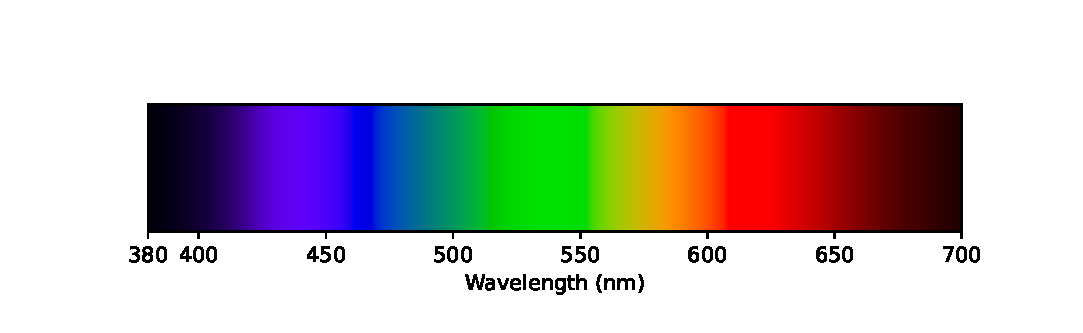
\includegraphics [angle=0, width=0.8\columnwidth] {fig/rgb.eps}
     \caption{\label{fig:rgb} RGB values obtained with $(\ref{eq:diracwavel})$.}
  \end {center}
\end {figure}

\subsection{Basic Radiometry}
\subsubsection{Black-Body Radiance}
\begin {figure}
  \begin {center}
     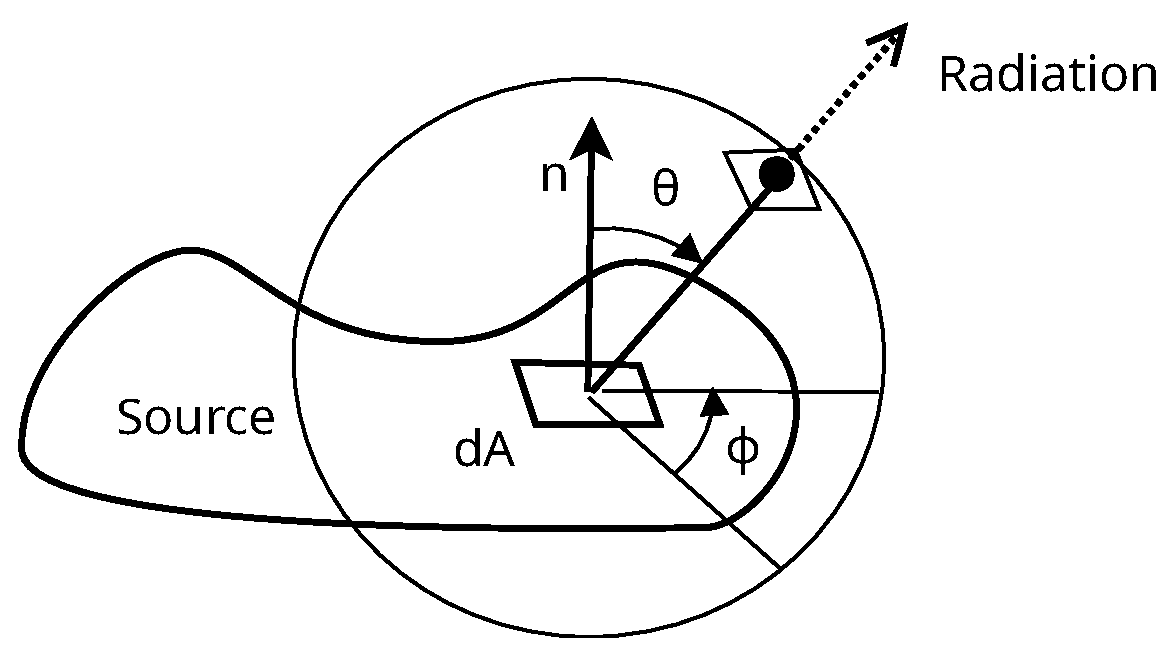
\includegraphics [angle=0, width=0.45\columnwidth] {fig/radiance.eps}
     \caption{\label{fig:radiance} Geometry associated to the definition of radiance.}
  \end {center}
\end {figure}
\textbf{Luminosity} (also called \textbf{radiant flux}) $L$ $(W)$ for a 
closed surface is an absolute measure of radiated electromagnetic energy 
per unit time. The luminosity of Sun is denoted $L_{\odot}$. 
\textbf{Radiance} for a source $L_e$ is the radiant flux from a given surface 
per unit projected area. That is, 
\begin {eqnarray}
    L_e 
    &=&
    \pdiff{}{\Omega}\pdiff{L}{A\cos\theta}
\end {eqnarray}
where $\Omega$ is the solid angle around the surface element $dA$, $A$ is 
the area on the source and $\theta\in[0, \pi/2]$ is the angle between the 
surface normal and the point on the unit sphere (see Figure \ref{fig:radiance}). 
Projection of an area element $dA$ to the direction $\theta$ w.r.t. surface 
normal is equal to $\cos\theta\:dA$.

\textbf{Spectral radiance} in frequency or wavelength are defined 
\begin {eqnarray}
    L_{e,\nu} := \pdiff{L_e}{\nu} 
    &\Leftrightarrow&
    L_e = \int_0^\infty L_{r,\nu}(\nu)\:d\nu
    \\
    L_{e,\lambda} := \pdiff{L_e}{\lambda} 
    &\Leftrightarrow&
    L_e = \int_0^\infty L_{r,\lambda}(\lambda)\:d\lambda,
\end {eqnarray}
respectively. 
Spectral radiance of a \textbf{black-body} can be written 
\begin{eqnarray}
    \label{eq:blackbody_specfreq}
    L_{e,\nu}(\nu) 
    &=&
    \frac{2h\nu^3}{c^2}
    \left[
        \exp\left({\frac{h\nu}{kT}}\right) - 1
    \right]^{-1}
    \\
    \label{eq:blackbody_specwave}
    L_{e,\lambda}(\lambda) 
    &=&
    \frac{2hc^2}{\lambda^5}
    \left[
        \exp\left({\frac{hc}{\lambda kT}}\right) - 1
    \right]^{-1},
\end{eqnarray} 
where 
$h=6.62607015\cdot 10^{-34}\:\textrm{J}\cdot\textrm{Hz}^{-1}$ is 
the \textbf{Planck's constant} and 
$k=1.380649\cdot{10}^{-23}\:\textrm{J}\cdot\textrm{K}^{-1}$ is the 
\textbf{Bolzmann constant}.
To obtain radiance, we integrate over all frequencies
\begin {eqnarray}
    L_e 
    &=&
    \frac{2h}{c^2}\int_0^\infty
    \frac{\nu^3\:d\nu}{\exp\left(\frac{h\nu}{kT}\right) - 1}
\end {eqnarray}
using the substitution $x=h\nu/kT$. Substituting correspondingly 
$\nu=kT/h\:x$ and $d\nu=kT/h\:dx$, we obtain 
\begin {eqnarray}
    L_e 
    =
    \frac{2h}{c^2}\left(\frac{kT}{h}\right)^4
    \int_0^\infty\frac{x^3\:dx}{e^x - 1}
    =
    \frac{2h}{c^2}\left(\frac{kT}{h}\right)^4 \Gamma(4)\zeta(4),
\end {eqnarray}
where $\Gamma$ and $\zeta$ are the Gamma and Riemann zeta functions.
Substitution of $\Gamma(4) = 6$ and $\zeta(4) = \pi^4/15$ yields 
\begin {eqnarray}
    \label{eq:blackbody_radiance}
    L_e 
    =
    \frac{2\:k^4\pi^4}{15\:h^3c^2}\:T^4.
\end {eqnarray}
To obtain the radiant flux, we integrate the radiance over a hemisphere
of solid angles and the entire surface 
\begin {eqnarray}
    L 
    &=&
    \oint_A\int_\Omega L_e(\vc r, \theta, \phi)\cos\theta\:d\Omega\:dA
\end {eqnarray}
where $\vc r$ is a point on the surface element $dA$. The computation of the 
integral is simplified by the intependence of radiance 
$(\ref{eq:blackbody_radiance})$ from $\theta$ and $\phi$. For solid angle,
we can expand $d\Omega = \sin\theta\:d\theta d\phi$. Thus, 
\begin {eqnarray}
    L 
    = 
    \oint_A L_e 
    \int_0^{2\pi}\int_0^{\pi/2}\sin\theta\cos\theta\:d\theta\:d\phi\:dA
    =
    \pi\oint_A L_e\:dA.
\end {eqnarray}
If $L_e$ is independent of position on the surface (e.g. due to equal 
temperature), we obtain 
\begin {eqnarray}
    L = \pi AL_e.
\end {eqnarray}
For a black-body
\begin {eqnarray}
    L 
    =
    \pi A L_e
    =
    \frac{2}{15}\frac{k^4\pi^5}{h^3c^2}AT^4 
    =
    \sigma AT^4, 
\end {eqnarray}
where the \textbf{Stefan-Boltzmann constant}
\begin {eqnarray}
    \sigma = \frac{2k^4\pi^5}{15h^3c^2} 
    = 
    5.670374419\cdot 10^{-8}\:\textrm{W}\cdot\textrm{m}^{-2}\cdot \textrm{K}^{-4}.
\end {eqnarray}
\subsubsection{Wien's Displacement Law}
To obtain peak frequency of the black body radiance as a function of temperature,
we derivate $(\ref{eq:blackbody_specfreq})$ w.r.t. frequency 
\begin{eqnarray}
    \pdiff{L_{e,\nu}}{\nu}
    =
    \frac{6h\nu^2}{c^2}
    \left[\exp\left(\frac{h\nu}{kT}\right) - 1\right]^{-1}
     - \frac{2h^2\nu^3}{c^2kT}\exp\left(\frac{h\nu}{kT}\right)
     \left[\exp\left(\frac{h\nu}{kT}\right) - 1\right]^{-2}
     = 0.
\end {eqnarray}
Substitution of $x=h\nu/kT$ yields 
\begin {eqnarray}
    x = 3(1 - e^{-x}),
\end {eqnarray}
which admits numerical solution
\begin {eqnarray}
    x = \frac{h\nu}{kT} \approx 2.821439372122078893
\end {eqnarray}
Thus, the blackbody radiance obtains it's peak at the frequency
and wavelength
\begin {eqnarray}
    \nu_{peak} 
    &=& 
    \frac{kT}{h}x \approx 5.878925757646824946 T\cdot 10^{10}
    \:\textrm{Hz}\cdot\textrm{K}^{-1}
    \\
    \label{eq:wien}
    \lambda_{peak} 
    &=&
    \frac{hc}{kTx}  
    \approx 2.897771955 / T\cdot 10^{-3}\:\textrm{m}\cdot\textrm{K}.
\end {eqnarray} 
The equation $(\ref{eq:wien})$ is called the \textbf{Wien's displacement law}
and is usually written in terms of the constant of proportionality $b=hc/kT$
called the \textbf{Wien's displacement constant}.

\subsection{Stars}
\subsubsection{Spectral Classification of Stars}
\subsubsection{Observed Spectral Power Distribution}
\subsubsection{Doppler Effect}

\subsection{Planets}

\newpage

\section{Visual Effects at Relativistic Speeds}
\subsection{Deformation}
\subsubsection{Grid Deformation}
\subsubsection{Solid Objects}
\subsection{Brightness}
\subsubsection{Headlight Effect}


\end {document}
